\chapter{Historia madżonga}
\label{historia}
% %%%%%%%%%%%%%%%%%%%%%%%%%%%%%%%%%%%%%%%%%%%%%%%%%%%%%%%%%%%%%%%%%%%%%%%%
% POCZĄTKI
% %%%%%%%%%%%%%%%%%%%%%%%%%%%%%%%%%%%%%%%%%%%%%%%%%%%%%%%%%%%%%%%%%%%%%%%%
\section{Początki madżonga}
% %%%%%%%%%%%%%%%%%%%%%%%%%%%%%%%%%%%%%%%%%%%%
% L.L. HARR
% %%%%%%%%%%%%%%%%%%%%%%%%%%%%%%%%%%%%%%%%%%%%%
\subsection{Mity na temat starożytnych początków madżonga}
Nie jest kwestią prostą ustalenie od którego momentu w historii możemy mówić o
madżongu. Sprawa ta jest tym trudniejsza, że wiele powszechnie dostępnych źródeł
zawiera informacje nieprecyzyjne lub wręcz całkowicie błędne. 

Niezwykle popularnym, choć niewiele mającym wspólnego z rzeczywistością, jest
pogląd, że madżong jest grą niezwykle starą, pamiętającą czasy Konfucjusza,
czyli V wiek przed naszą erą. Ów pogląd wywodzi się z niesławnej publikacji Lew
Lysle Harra wydanej w 1922 roku pod tytułem ,,Pung Chow''\footnote{Tytuł książki
L.L. Harra ,,Pung Chow'' to jedna z popularniejszych nazw, jaką określano
madżonga w pierwszej połowie XX wieku. ,,Pung'' i ,,chow'' to przyjęty przez
Harra zapis 2 spośród najpopularniejszych ruchów dozwolonych w madżongu --
współcześnie są one znane jako \pinyin{peng} (碰 pèng) i \pinyin{chi} (吃 chī).}
(Harr 2008).
Lew Lysle Harr był w Chinach w 1919 roku reprezentantem amerykańskiej firmy
Graton and Knight Belting Company. Uznał on, że masowo produkowane zestawy do
madżonga w zunifikowanej, jednolitej formie pozwoliłoby na łatwą wymianę
zgubionych kamieni oraz byłyby łatwiejsze do sprzedaży.
Wyżej wymieniona publikacja to spisany przez niego podręcznik do nauki zasad
gry, który w swoim wstępie zawiera notatkę o historii i pochodzeniu madżonga.
Według jej treści, madżong w swojej pierwotnej postaci wymyślony został około
472 roku przed naszą erą na dworze króla państwa Wu, czyli w okolicach
współczesnego Ningbo\footnote{Ningbo (宁波 \pinyin{Níngbō}) - miasto we
wschodnich Chinach, w prowincji Zhejiang (浙江 \pinyin{Zhèjiāng}), port handlowy i
rybacki nad Morzem Wschodniochińskim.}. Madżong miał tam funkcjonować pod nazwą
\textit{Pe-Ling} jako gra umilająca czas samemu królowi, jego rodzinie i
bliskiemu otoczeniu. Karą za spędzanie w ten sposób czasu przez niższe warstwy
społeczeństwa była śmierć poprzez ścięcie głowy. Później dostęp do gry miał
zostać rozszerzony do kasty kupców, a dopiero w połowie XIX wieku naszej ery
stać się powszechnie dostępnym.
Publikacja prezentująca powyższe informacje miała służyć reklamie produktu,
który L.L. Harr zamierzał sprzedawać. Jako że zgodnie z ówczesnymi (jak
też i współczesnymi) badaniami nad pochodzeniem madżonga, gra nie istniała przed
XIX wiekiem naszej ery, a cała historia podana we wstępie do ,,Pung Chow'' była
nieprawdziwa, książka spotkała się z ostrą krytyką, a firma Harra zbankrutowała
w 1925 roku. Jednakże, choć L.L. Harr nie odniósł sukcesu w dziedzinie sprzedaży
madżonga, jego książka jest współcześnie powszechnie dostępna w księgarniach, a
ostra krytyka, z jaką się spotkała zaraz po jej pierwszej publikacji nie jest
wiedzą powszechną. W wyniku tego, że Harr faktycznie znajdował się w Chinach w
latach dwudziestych XX wieku, gdy madżong po raz pierwszy zaczął trafiać do
szerokiej publiczności w Europie i Ameryce Północnej, wiele źródeł uznaje jego
książkę za wiarygodną i odnosi się do zawartych w niej fałszywych informacji
(Greenfield 2010; Harr 2008; Mah Jong Museum).
% %%%%%%%%%%%%%%%%%%%%%%%%%%%%%%%%%%%%%%%%%%%%
% FAKTYCZNE POCZĄTKI
% %%%%%%%%%%%%%%%%%%%%%%%%%%%%%%%%%%%%%%%%%%%%%
\subsection{Gry karciane - rzeczywiste początki madżonga}
Nawet po eliminacji źródeł zawierających informacje niewątpliwie fałszywe,
ustalenie dokładnego momentu pojawienia się madżonga po raz pierwszy pozostaje
kwestią trudną. Częścią problemu jest fakt, że już wtedy, gdy pierwszy raz
zaczęto używać nazwy ,,madżong'', nie była to gra całkowicie nowa, lecz raczej
kombinacja zasad szeregu funkcjonujących na terenie Chin w XIX wieku i wcześniej
hazardowych gier karcianych. 

%dopisany fragment podpierający to, ze w Chinach o hazardzie pisać było wstyd
%i stąd jest mało chińskich źródeł
Sprawa okazuje się być tym bardziej skomplikowana w związku z długą historią
uprawiania hazardu, który był w Chinach popularny już od czasów starożytnych.
Pierwsze odnotowane przypadki jego uprawiania sięgają końca dynastii Zhou (周
Zhōu) (między 800 a 256 rokiem przed naszą erą), jednakże niektórzy historycy
sugerują, że faktycznie do pierwszych takich zajść mogło dochodzić już za
dynastii Shang (商 Shāng)(między 1700 a 1027 rokiem przed naszą erą), a nawet Xia
(夏 Xià) (między 2000 a 1500 rokiem przed naszą erą). Od tego czasu chińscy
władcy wielokrotnie próbowali kontrolować te zjawiska, a nawet całkowicie
zakazywać hazardu, jednakże nie były to rozwiązania trwałe aż do całkowitego
zakazu wprowadzonego w roku 1966. Przykładowo, choć Zhu Yuanzhang (朱元璋 Zhū
Yuánzhāng), pierwszy cesarz dynastii Ming (明 Míng) w latach 1368-1398, zakazał
hazardu na początku swoich rządów, sam nie przestrzegał własnego rozporządzenia,
grając często na pieniądze ze swoimi współpracownikami (Tse, Samson \& Yu, Alex
C.H. \& Rossen, Fiona \& Wang, Chong-Wen 2010).

Mimo że przez tysiące lat hazard pozostawał popularnym sposobem spędzania czasu
dla wszystkich warstw społeczeństwa, nie był on w żadnym razie powodem do dumy.
Jedno z chińskich źródeł traktujących o hazardzie pochodzące z 1783 roku, do
których odnosi się niniejsza praca, zostało zatytułowane ,,Plotki o
Świniopasach'' (牧猪闲话 \pinyin{Mùzhū Xiánhuà}), co zwraca uwagę na to, w jaki
sposób jego autor, Jin Xueshi (金学诗 Jīn Xuéshī), traktował ten temat.  W czasie,
gdy starsze gry karciane powoli przekształcały się w grę nazywaną ,,madżongiem''
wzbudzało to w większym stopniu zainteresowanie naukowców napływających z
Ameryki Północnej i Europy, niż tych pochodzących z Chin. Jako że pierwsi uczeni
publikujący na ten temat w drugiej połowie XIX wieku nie zajmowali się
ustaleniem historycznych początków madżonga, lecz raczej próbowali przedstawić
społeczeństwu zachodniemu, wiele dat podawanych przez autora w dalszej części
tego rozdziału jest jedynie przybliżeniem na podstawie powstałych dużo później
rekonstrukcji.

% %%%%%%%%%%%%%%%% GRY KARCIANE
Jednakże, przed ustaleniem momentu pojawienia się madżonga należy poświęcić
uwagę również grom karcianym, z których prawdopodobnie się on wywodzi.

% %%%%%%%%%%%%%%%% SHIHU
Jedną z nich, która uznawana jest za spokrewnioną z madżongiem, jest
\pinyin{shihu} (十壶 \pinyin{shíhú}). Nazwę można by dosłownie przetłumaczyć jako
,,10 dzbanków'', choć spotykane jest także tłumaczenie ,,10 punktów'' (Stanwick,
Xu za Lo 2004). Można zatem przypuścić, że nazwę gry można również zapisać 十和
(\pinyin{shíhú}\footnote{Choć najczęstsze czytanie znaku 和 to ,,\pinyin{hé}'', a
znak ten najczęściej oznacza pokój, harmonię, a także występuje w zdaniu jako
spójnik, w kontekscie madżonga i wielu spokrewnionych z nim gier czytany jest on
,,\pinyin{hú}''. Oznacza on wówczas skompletowanie ręki, czyli zwycięstwo w
rozdaniu. Analogicznie, prawdopodobnie najcelniejszym tłumaczeniem \pinyin{mohu}
(patrz: strona \pageref{mohu_page}) jest ,,kompletowanie ręki w milczeniu''.}),
czyli dosłownie ,,10 wygranych''. Do gry służył zestaw kart papierowych, których
liczba zazwyczaj wynosiła 120, choć można było również spotkać warianty na 125,
132, a nawet 160 kart. Zestaw składał się z:
\begin{itemize}
  \item 36 kart (4 egzemplarze każdego rodzaju karty) w każdej z 3 talii (餅
  \pinyin{bǐng}, 索 \pinyin{suǒ} oraz 万 \pinyin{wàn}), łącznie 108 kart;
  \item po 4 egzemplarze 3 kart kwiatów (花 \pinyin{huā}), łącznie 12 kart;
  \item rzadziej innych dodatkowych kart.
\end{itemize}
Jak łatwo zauważyć, choć skład takiego zestawu nie spełnia norm przyjętych w
madżongu, jest do nich bardzo zbliżony. Oznaczenia na kartach również odbiegają
od tych stosowanych w madżongu (Rysunek \ref{fig:zestawshihu}).
Sama gra w \pinyin{shihu}, podobnie jak gra w madżonga, polegała na ułożeniu określonego układu w procesie
dobierania i odrzucania kart przez graczy po kolei. Zwycięski układ musiał być
wart minimum 10 punktów. \pinyin{Shihu} niewątpliwie zostało wymyślone przed
madżongiem, jako że jest wspominane w dziele pochodzącym z 1796 roku --
,,Malowane Łodzie Przyjemności z Yangzhou''\footnote{Tytułowe ,,łodzie
przyjemności'' to domy publiczne w Yangzhou (扬州 \pinyin{Yángzhōu}), mieście we
wschodnich Chinach. Klienci owych domów publicznych grywali w \pinyin{shihu},
nie jest jednakże jasnym, czy była to usługa świadczona przez same instytucje,
czy też zwyczajnie popularna w ich gronie rozrywka (Stanwick \& Xu).}
autorstwa \pinyin{Li Dou} (李斗, \pinyin{Lǐ Dǒu}) (Stanwick \& Xu).

\begin{figure}[h]
\centering
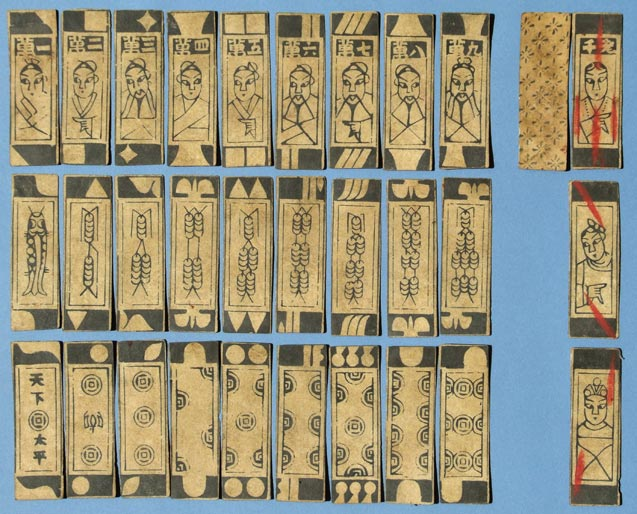
\includegraphics[width=0.75\textwidth]{1_shihu.jpg}
\caption{Niekompletny zestaw do gry w \pinyin{shihu}; 30 spośród 120 kart;
Chiny, ok. 1900 r;  źródło:
http://www.themahjongtileset.co.uk/tile-set-history/earliest-suit-names/}
\label{fig:zestawshihu}
\end{figure}

% MADIAO
Same karty używane do gry w \pinyin{shihu} wykorzystywane były również do wielu
innych gier, a ich wcześniejszym zastosowaniem prawdopodobnie była gra w
\pinyin{madiao} (馬吊 \pinyin{mǎdiào}), czyli dosłownie ,,wieszanie konia'',
pochodząca z czasu rządów cesarza Kangxi (康熙 Kāngxī), czyli z lat 1661--1722.
(Jin 1783) Zestaw \pinyin{madiao} składał się z 40 kart w 4 taliach -- czwarta
talia, niewystępująca w grach wywodzących się z \pinyin{madiao}, nazywana była
,,dziesiątkami myriad'' (万贯 \pinyin{wànguàn}). Później wykorzystywano zestawy
zawierające tylko 3 talie (czyli 30 kart) do innych gier (Stanwick \& Xu).

%MOHU
\label{mohu_page}
Przykładem innej gry wykorzystującej zestaw do \pinyin{madiao} jest
\pinyin{mohu} (默和 \pinyin{mòhú}). Gra była przeznaczona dla			
% tu było tłumaczenie, czym jest mohu, ale zostało przy shihu kawałek wcześniej
4 graczy i wymagała 60 kart (czyli najprawdopodobniej 2 zestawów kart
\pinyin{madiao} pozbawionych talii dziesiątków myriad). Jeden z graczy rozdawał
wszystkim uczestnikom po kolei po 1 karcie, aż każdy miał ich po 10. Następnie
gracze układali je w ciszy. Dalsza rozgrywka polegała na dobieraniu kart z
pozostałych 20 w celu ułożenia zwycięskiego układu (jeden z graczy, ale nie ten
odpowiadający za pierwsze rozdanie kart, rozdawał kolejne) (Jin 1783; Stanwick
\& Xu).
% 
% \footnote{,,Natrafianie na układ z
% kart'' to dosłowne znaczenie nazwy \pinyin{penghu}, jednakże prawdopodobnie jej
% pochodzenie jest nieco inne. \pinyin{Peng} (碰 \pinyin{pèng}) to jedna z
% najczęściej stosowanych deklaracji we współczesnym madżongu. Jej użycie pozwala
% na dobranie kamienia odrzuconego przez innego gracza do własnej trójki takich
% samych kamieni. Prawdopodobnie zachodzi związek pomiędzy tą nazwą, a nazwą gry w \pinyin{penghu}.}


% PENGHU
Inną tego typu grą jest \pinyin{penghu} (碰和 \pinyin{pènghú} -- dosłownie
,,natrafianie na układ z kart'').
W \pinyin{penghu} grano 4 lub 5 zestawami do \pinyin{madiao}, czyli łącznie 120
lub 150 kartami (Stanwick \& Xu). Inne źródło sugeruje, że stosowano 2 lub 2,5
zestawu do \pinyin{mohu} (Jin 1783), co sumuje się do tej samej liczby kart.
Nie jest oczywistym, czy gra wykształciła się bezpośrednio z \pinyin{madiao},
czy też pośrednio z \pinyin{mohu} (jak sugeruje Jin 1783).
Pojawiają się w niej układy występujące również we współczesnym madżongu, jak na
przykład \pinyin{peng}\footnote{\pinyin{peng} (碰 \pinyin{pèng}) to jedna z
 najczęściej stosowanych deklaracji we współczesnym madżongu. Jej użycie pozwala
 na dobranie kamienia odrzuconego przez innego gracza do własnej trójki takich
 samych kamieni. Występuje również w grze w \pinyin{penghu} i jest elementem jej
 nazwy.}. Można sądzić, że niektóre źródła mowiące tylko o \pinyin{shihu} lub
 tylko o \pinyin{penghu} nie rozróżniały tych dwóch gier, jako że ich zasady i
 skład zestawów do gry były do siebie zbliżone (Jin 1783; Stanwick \& Xu).

% PODSUMOWANIE KART
Karty do \pinyin{madiao} były również wykorzystywane do szeregu innych,
pomniejszych gier, jak \pinyin{kanhu} (看虎 \pinyin{kànhǔ} \label{kanhu}--
,,obserwowanie tygrysa''), \pinyin{hunjiang} (混江 \pinyin{hùnjiāng} -- ,,zwijanie rzeki'') oraz
\pinyin{suohu} (梭和 \pinyin{suōhú} - ,,układanie kart ruchem w tę i z
powrotem'') (Stanwick \& Xu). Każda z nich jest warta wspomnienia, jako że wielu
pasjonatów oraz badaczy na przełomie XIX i XX wieku określało własne zestawy do
madżonga właśnie ich nazwami (nie będąc jeszcze świadomym różnicy).
Można wręcz przypuszczać, że funkcjonowały one przez długi czas równolegle z
nowo wykształconym madżongiem, a być może nawet grano w nie przy pomocy
kamieni zamiast kart.
% %%%%%%%%%%%%%%%%%%%%%%%%%%%%%%%%%%%%%%%%%%%%
% MADŻONG NA PRZEŁOMIE XIX/XX WIEKU
% %%%%%%%%%%%%%%%%%%%%%%%%%%%%%%%%%%%%%%%%%%%%%
\subsection{Madżong pod koniec XIX wieku}
Ciężko określić, w którym dokładnie momencie zaczęto używać kamieni do gry
zamiast kart\footnote{Ze względu na nierozróżnianie ich w języku i określanie
wspólnym mianem \pinyin{pai}, zgodnie z zapisem w sekcji 1.1.2.}, jednakże było
to już niewątpliwie praktykowane w latach siedemdziesiątych XIX wieku (Stanwick
2004). Niemiecki tłumacz Carl Himly w latach 1868-1876 zdobył zestaw bambusowych
kamieni, które w swoich publikacjach z 1889 i 1901 określał jako ,,bambusowe
\pinyin{pai} z Ningbo\footnote{Ningbo (宁波 \pinyin{Níngbō}) -- miasto we
wschodnich Chinach, w prowincji Zhejiang (浙江 Zhèjiāng), port handlowy i rybacki
nad Morzem Wschodniochińskim.}'' (宁波竹牌 \pinyin{Níngbō zhúpái}). Nie spełnia on
definicji madżonga przyjętej na potrzeby tej pracy (brakuje w nim kamieni
czerwonego oraz zielonego smoka), jednakże jest do niej bardzo zbliżony
(Stanwick, Xu za Himly 1889-1901). Bardzo podobne zestawy (w których
uwzględniony już został smok czerwony, jednakże wciąż brakowało zielonego)
pochodzące z okresu pomiędzy 1869 a 1875 rokiem zostały dostarczone przez
George'a B. Glovera\footnote{George B. Glover, wicekonsul Stanów Zjednoczonych w
Szanghaju w latach 1858-1859. Później w latach od 1859 do około 1882 komisarz
urzędu celnego w różnych miejscach w Chinach (Wikipedia 2013).} do
Amerykańskiego Muzeum Historii Naturalnej (American Museum of Natural History)
(Stanwick 2004). Glover napisał w 1875 roku notatkę, która została załączona do
owych zestawów, w której prawdopodobnie po raz pierwszy użyto poza Chinami nazwy
,,wróbel''\footnote{Glover w 1975 roku użył nazwy \pinyin{jiaqiao} (家雀
\pinyin{jiāqiǎo}), czyli dosłownie ,,wróbel domowy''. Współcześnie łatwiej można
spotkać określenie \pinyin{maque} (麻雀 \pinyin{máquè}), które również oznacza
wróbla, jednakże regionalnie można wciąż spotkać się także z użyciem tego słowa
jako synonim madżonga. W języku japońskim \pinyin{majian}, które zapisywane jest
tymi samymi znakami, co \pinyin{maque} po chińsku, również oznacza madżonga
(Stanwick \& Xu).}, która współcześnie jest jednym z wielu synonimów madżonga.
Zestawy różniły się pomiędzy sobą składem, jednakże można przyjąć że służyły do
tych samych lub spokrewnionych ze sobą gier. Jako że pochodziły z różnych
obszarów Chin -- Ningbo i Szanghaju, stosowanie zestawów kamieni zamiast kart
prawdopodobnie stawało się w tym czasie coraz bardziej popularne w Chinach.

Bardziej precyzyjne badania nad madżongiem rozpoczynają się w roku 1893, kiedy
to William Henry Wilkinson, pracownik konsulatu brytyjskiego w Chinach, wysłał
zbiór gier zakupionych w Chinach do profesora Stewarta Culina,\footnote{Stewart
Culin, amerykański etnograf, pracownik Uniwersytetu Pensylwanii, badacz gier,
ubioru i sztuki chińskiej; jeden z pierwszych badaczy madżonga (Wikipedia
2016).} który Culin później wystawił na wystawie World's Colombian Exposition w
Chicago. W owym zbiorze znajdowała się gra karciana, którą Wilkinson określał
jako \pinyin{khanhoo}, czyli najprawdopodobniej wspomniane na stronie
\pageref{kanhu} \pinyin{kanhu} (看虎 \pinyin{kànhǔ} -- ,,obserwowanie tygrysa'').
\pinyin{Khanhoo}, pośród innych gier wymienianych przez Wilkinsona, należało do
podzbioru określanego przez niego mianem ,,wróbli'', czyli \pinyin{maque}. Culin
zajął się badaniami na ten temat i w późniejszych publikacjach uznał ,,wróble''
Wilkinsona za przodków madżonga (Culin 1924; Greenfield 2010).

% %%%%%%%%%%%%%%%%%%%%%%%%%%%%%%%%%%%%%%%%%%%%
% XX WIEK
% %%%%%%%%%%%%%%%%%%%%%%%%%%%%%%%%%%%%%%%%%%%%%
\section{Madżong w XX wieku}

% %%%%%%%%%%%%%%%%%%%%%%%
% SZANGHAJ 20s
% %%%%%%%%%%%%%%%%%%%%%%%
\subsection{Madżong w Szanghaju lat dwudziestych XX wieku}
\label{shanghai20s}
Jakkolwiek \pinyin{khanhoo} cieszyło się zainteresowaniem naukowców, poza
terenem Chin nie zdobyło popularności. Przełomowy moment w historii madżonga nastąpił wtedy,
gdy gra trafiła do Szanghaju. Choć zasady sformułowane zostały w Ningbo, to
Szanghaj pozwolił im się w pełni rozwinąć i trafić do szerszego grona odbiorców.
W wyniku traktatów podpisanych po zakończeniu dziewiętnastowiecznych Wojen
opiumowych\footnote{Wojny opiumowe – wspólne określenie na mające miejsce w
dziewiętnastym wieku 2 konflikty zbrojne Chin z Wielką Brytanią i Francją;
jednym z ich skutków był szereg upokarzających dla Chin traktatów wymuszających
ustępstwa handlowe przy handlu wieloma towarami, przede wszystkim opium.}, port
w Szanghaju stanowił jedną ze specjalnie wyznaczonych stref, gdzie przybysze ze
Stanów Zjednoczonych, Wielkiej Brytanii i innych państw zachodnich mogli
dokonywać swobodnej wymiany kulturowej, niepodlegając chińskiemu prawu oraz
podatkom (Greenfield 2010).

Sam Culin w 1909 roku w Szanghaju kupił \mbox{„zestaw
domina wykonany z kości słoniowej”,} który już spełniał definicję madżonga
opisaną na stronie \pageref{definicja}. Możemy przyjąć, że wówczas podobne
zestawy nie miały jeszcze ustalonego składu, jako że według informatora nazwiskiem Dzau Sing
Chung z Szanghaju, na którego powołuje się Culin, były one
zazwyczaj wykonywane na zamówienie, zgodnie z potrzebami klienta (Culin 1924).

Jednakże, dopóki zestaw do gry nie miał ustalonego składu i był wykonywany na
zamówienie, jego dystrybucja pozostawała problematyczna, w związku z czym szereg
osób dokonywało prób jego standaryzacji. Jedną z takich osób był Joseph A.
Babcock, reprezentant amerykańskiej firmy Standard Oil Company, który właśnie w
Szanghaju nauczył się grać w madżonga, by później
stać się najważniejszą osobą w historii popularyzacji tej gry na świecie. W
1920 roku wydał on pierwsze zasady gry w języku
angielskim, czyli ,,Czerwoną Księgę Zasad'' (\textit{Red Book of Rules}).
Książkę sprzedawano razem z zestawami do gry, którą początkowo importowano z
Chin, a później także wykonywano w Stanach Zjednoczonych. Babcock opatentował
nazwę ,,Mah-Jongg'', której różne pisownie (,,mahjong'', ,,majong'' i im
podobne) stały się powszechnie używaną na zachodzie nazwą gry. Określenie
,,madżong'', przyjęte na potrzeby niniejszej pracy, również jest jej
spolszczeniem. Wielu próbowało imitować sukces Babcocka, jednakże było
zmuszonych używać innych nazw gry, między innymi przez co nie odnieśli
porównywalnego sukcesu\footnote{Dla przykładu, wspomniany w sekcji 1.2.1 Lew
Lysle Harr był zmuszony używać nazwy ,,Pung Chow''.} (Greenfield 2010).

\subsection{Odrodzenie madżonga}
\label{zakaz_1966}
Jako że madżong w swojej pierwotnej postaci był grą hazardową, kojarzącą się z
rozwiązłym stylem życia zepsutego zachodu, został on zakazany w 1966 roku na
początku rewolucji kulturalnej\footnote{Wielka proletariacka rewolucja
kulturalna (无产阶级文化大革命 \pinyin{Wúchǎnjiējí} \pinyin{Wénhuà} \pinyin{Dàgémìng}) --
mający miejsce w latach 1966-1976 ruch społeczno-polityczny zapoczątkowany przez
przywódcę Partii Komunistycznej Chin, Mao Zedonga.}, wraz z wszystkimi innymi
przejawami hazardu na terenie całego kraju (Carlisle 2009).

\label{relegalizacja}
Stworzono nowe zasady, które miały wyeliminować elementy gry hazardowej i
uzyskać grę, w której najważniejsze byłyby umiejętności gracza. Tym samym, w
1998 roku opublikowano ,,Międzynarodowy Standard Madżonga'' (国际标准麻将
\pinyin{guójì biāozhǔn májiàng}), czyli międzynarodowe zasady turniejowe (w
poszechnym użytku jest skrót -- 国标麻将 \pinyin{guóbiāo} \pinyin{májiàng}), a zakaz
gry został zniesiony (szczegółowy opis wymienionych zasad znajduje się na stronie
\pageref{guobiao}).
W tym samym roku madżong został w Chinach oficjalnie uznany za dyscyplinę sportową (Carlisle 2009; Zi 2015).

\label{pierwsze_mistrzostwa}
W 2002 roku w Tokio odbyły się pierwsze na świecie międzynarodowe zawody w grze
w madżonga, na których obowiązywały już zasady \pinyin{guóbiāo}
\pinyin{májiàng}. Pierwotnie miały się one odbyć w Ningbo. Zwyciężył w nich
reprezentant Japonii, Mai Hatsune (Kanazawa 2010, Nihon kenkō asa shō kyōkai
kōshiki saito 2002).

\label{wmo}
W październiku 2005 roku w Pekinie utworzono Światową Organizację Madżonga
(World Mahjong Organization lub 世界麻将组织 \pinyin{Shìjiè Májiàng Zǔzhī}).
Poza Chinami, do krajów założycielskich należały między innymi Japonia, Stany
Zjednoczone Ameryki Północnej, Niemcy, Francja, Dania, Holandia oraz Węgry
(Shìjiè Májiàng Zǔzhī 2014).

W listopadzie 2007 roku w Chengdu\footnote{成都 (\pinyin{Chéngdū}) -- stolica
prowincji 四川 (\pinyin{Sìchuān}), miasto w południowo-wschodnich Chinach.} odbyły
się pierwsze oficjalne Światowe Mistrzostwa Madżonga. Od tego czasu stało się to
regularnym wydarzeniem - kolejne miały miejsce w 2010 roku w
Utrecht\footnote{Utrecht --  miasto w środkowej Holandii.} oraz w 2012 w
Chongqing\footnote{重庆 (\pinyin{Chóngqìng}) -- miasto w środkowych Chinach, jedno
z czterech miast wydzielonych Chińskiej Republiki Ludowej.} (Kǒuzhuāng Bāshì
2014).






 














